\documentclass[tikz,border=5pt]{standalone}
\usepackage{pgfplots}
\pgfplotsset{compat=1.18}
\usepackage{fontspec}
\setsansfont{SourceSansPro}[
  Path = /usr/local/texlive/2024/texmf-dist/fonts/opentype/adobe/sourcesanspro/,
  UprightFont = SourceSansPro-Regular.otf,
  BoldFont = SourceSansPro-Bold.otf,
  ItalicFont = SourceSansPro-RegularIt.otf,
  BoldItalicFont = SourceSansPro-BoldIt.otf,
  Scale = 1.0
]
\usetikzlibrary{positioning}
\usepackage{xcolor}
\definecolor{primaryblue}{HTML}{012169}
\definecolor{primarygold}{HTML}{B9975B}
\definecolor{highlightyellow}{HTML}{F2A900}
\definecolor{lightbg}{HTML}{E8EDF5}
\definecolor{jet}{HTML}{1A1A1A}
\definecolor{positivegreen}{HTML}{15803D}
\definecolor{negativered}{HTML}{B91C1C}
\begin{document}
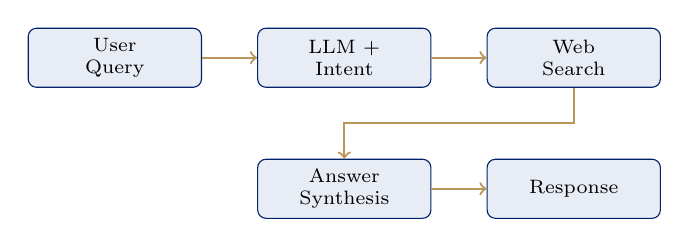
\begin{tikzpicture}[
  node distance=0.7cm,
  box/.style={draw=primaryblue, fill=lightbg, rounded corners=3pt,
              minimum width=2.2cm, minimum height=0.75cm,
              font=\scriptsize, align=center},
  arr/.style={->, thick, color=primarygold}
]
  % Row 1
  \node[box] (q)  {User\\Query};
  \node[box, right=of q]  (c)  {LLM +\\Intent};
  \node[box, right=of c]  (ws) {Web\\Search};

  % Row 2 — centered under row 1
  \node[box, below=0.9cm of c] (syn) {Answer\\Synthesis};
  \node[box, right=of syn]     (r)   {Response};

  % Row 1 arrows
  \draw[arr] (q)  -- (c);
  \draw[arr] (c)  -- (ws);

  % Bent arrow: ws down then left to syn
  \draw[arr] (ws.south) -- ++(0,-0.45) -| (syn.north);

  % Row 2 arrow
  \draw[arr] (syn) -- (r);
\end{tikzpicture}
\end{document}
